% Options for packages loaded elsewhere
\PassOptionsToPackage{unicode}{hyperref}
\PassOptionsToPackage{hyphens}{url}
%
\documentclass[
]{article}
\usepackage{amsmath,amssymb}
\usepackage{lmodern}
\usepackage{iftex}
\ifPDFTeX
  \usepackage[T1]{fontenc}
  \usepackage[utf8]{inputenc}
  \usepackage{textcomp} % provide euro and other symbols
\else % if luatex or xetex
  \usepackage{unicode-math}
  \defaultfontfeatures{Scale=MatchLowercase}
  \defaultfontfeatures[\rmfamily]{Ligatures=TeX,Scale=1}
\fi
% Use upquote if available, for straight quotes in verbatim environments
\IfFileExists{upquote.sty}{\usepackage{upquote}}{}
\IfFileExists{microtype.sty}{% use microtype if available
  \usepackage[]{microtype}
  \UseMicrotypeSet[protrusion]{basicmath} % disable protrusion for tt fonts
}{}
\makeatletter
\@ifundefined{KOMAClassName}{% if non-KOMA class
  \IfFileExists{parskip.sty}{%
    \usepackage{parskip}
  }{% else
    \setlength{\parindent}{0pt}
    \setlength{\parskip}{6pt plus 2pt minus 1pt}}
}{% if KOMA class
  \KOMAoptions{parskip=half}}
\makeatother
\usepackage{xcolor}
\usepackage[margin=1in]{geometry}
\usepackage{longtable,booktabs,array}
\usepackage{calc} % for calculating minipage widths
% Correct order of tables after \paragraph or \subparagraph
\usepackage{etoolbox}
\makeatletter
\patchcmd\longtable{\par}{\if@noskipsec\mbox{}\fi\par}{}{}
\makeatother
% Allow footnotes in longtable head/foot
\IfFileExists{footnotehyper.sty}{\usepackage{footnotehyper}}{\usepackage{footnote}}
\makesavenoteenv{longtable}
\usepackage{graphicx}
\makeatletter
\def\maxwidth{\ifdim\Gin@nat@width>\linewidth\linewidth\else\Gin@nat@width\fi}
\def\maxheight{\ifdim\Gin@nat@height>\textheight\textheight\else\Gin@nat@height\fi}
\makeatother
% Scale images if necessary, so that they will not overflow the page
% margins by default, and it is still possible to overwrite the defaults
% using explicit options in \includegraphics[width, height, ...]{}
\setkeys{Gin}{width=\maxwidth,height=\maxheight,keepaspectratio}
% Set default figure placement to htbp
\makeatletter
\def\fps@figure{htbp}
\makeatother
\setlength{\emergencystretch}{3em} % prevent overfull lines
\providecommand{\tightlist}{%
  \setlength{\itemsep}{0pt}\setlength{\parskip}{0pt}}
\setcounter{secnumdepth}{5}
\newlength{\cslhangindent}
\setlength{\cslhangindent}{1.5em}
\newlength{\csllabelwidth}
\setlength{\csllabelwidth}{3em}
\newlength{\cslentryspacingunit} % times entry-spacing
\setlength{\cslentryspacingunit}{\parskip}
\newenvironment{CSLReferences}[2] % #1 hanging-ident, #2 entry spacing
 {% don't indent paragraphs
  \setlength{\parindent}{0pt}
  % turn on hanging indent if param 1 is 1
  \ifodd #1
  \let\oldpar\par
  \def\par{\hangindent=\cslhangindent\oldpar}
  \fi
  % set entry spacing
  \setlength{\parskip}{#2\cslentryspacingunit}
 }%
 {}
\usepackage{calc}
\newcommand{\CSLBlock}[1]{#1\hfill\break}
\newcommand{\CSLLeftMargin}[1]{\parbox[t]{\csllabelwidth}{#1}}
\newcommand{\CSLRightInline}[1]{\parbox[t]{\linewidth - \csllabelwidth}{#1}\break}
\newcommand{\CSLIndent}[1]{\hspace{\cslhangindent}#1}
\newcommand{\beginappendix}{ \setcounter{table}{0} \renewcommand{\thetable}{A\arabic{table}} \setcounter{figure}{0} \renewcommand{\thefigure}{A\arabic{figure}} }
\usepackage[capposition=top]{floatrow}
\usepackage{placeins}
\usepackage{setspace}
\usepackage{dcolumn}
\usepackage{booktabs}
\usepackage{siunitx}
\usepackage{amsmath}
\usepackage{enumerate}
\usepackage[shortlabels]{enumitem}
\usepackage[hang,flushmargin]{footmisc}
\usepackage{makecell}
\usepackage{booktabs}
\usepackage{longtable}
\usepackage{array}
\usepackage{multirow}
\usepackage{wrapfig}
\usepackage{float}
\usepackage{colortbl}
\usepackage{pdflscape}
\usepackage{tabu}
\usepackage{threeparttable}
\usepackage{threeparttablex}
\usepackage[normalem]{ulem}
\usepackage{makecell}
\usepackage{xcolor}
\ifLuaTeX
  \usepackage{selnolig}  % disable illegal ligatures
\fi
\IfFileExists{bookmark.sty}{\usepackage{bookmark}}{\usepackage{hyperref}}
\IfFileExists{xurl.sty}{\usepackage{xurl}}{} % add URL line breaks if available
\urlstyle{same} % disable monospaced font for URLs
\hypersetup{
  pdftitle={Pollution, agricultural productivity, and development: Evidence from coal plants in India},
  pdfauthor={Joshua D. Merfeld},
  hidelinks,
  pdfcreator={LaTeX via pandoc}}

\title{Pollution, agricultural productivity, and development: Evidence from coal plants in India\footnote{I thank Marc Bellemare and David Sungho Park for comments and suggestions that greatly improved the quality of the paper. The usual disclaimer applies. All scripts used in this paper are publicly available on my GitHub page: github.com/JoshMerfeld/pollution\_development}}
\author{Joshua D. Merfeld\footnote{KDI School of Public Policy and Management and IZA; \href{mailto:merfeld@kdis.ac.kr}{\nolinkurl{merfeld@kdis.ac.kr}}}}
\date{2023-02-10}

\begin{document}
\maketitle
\begin{abstract}
\noindent I show that emissions from a common energy source lead to decreased productivity and growth. The rapid increase in population in India from the 1990s through the 2010s led to the rapid construction of new coal power plants throughout the country. Using this roll-out combined with random changes in wind direction, I document negative effects of pollution from coal power plants on agricultural productivity throughout the country. Results suggest this decrease may be driven by a decline in labor allocation of the oldest half of my sample, who greatly decrease labor allocated to both farm and non-farm employment when exposed to pollution. These impacts spill over into aggregate economic growth, as well; nightlight growth is slower following years of higher exposure to pollution.\\
\strut \\
\textbf{\textit{Keywords}}: pollution, productivity, agriculture, labor, India\\
\textbf{\textit{JEL Codes}}: H40, I15, J22, O13, Q52, Q53
\end{abstract}

\newpage
\doublespacing

\hypertarget{introduction}{%
\section{Introduction}\label{introduction}}

Coal is one of the most common energy sources throughout the world. In 2021, energy generation from coal reached an all-time high,\footnote{www.iea.org/reports/coal-fired-electricity} driven in part by rapid population growth and rising energy prices. India is no exception to these trends. From 1990 to 2010, India's population grew by more than 40 percent.\footnote{data.worldbank.org} This population growth led to a large increase in demand for power. While natural gas has become a popular alternative in much of the world, the Indian government met much of the increased demand through the construction of coal power plants. During those same two decades, power generation from all coal units of at least 30 megawatts in the country increased by almost 140 percent, from 42.4 gigawatts to more than 100 gigawatts.\footnote{globalenergymonitor.org/} There are no doubt positive effects from this increase in power generation; for example, electricity may lead to economic and productivity growth (Dinkelman 2011; Kline and Moretti 2014; Rud 2012; Van de Walle et al. 2017), though electrification alone may not be a sufficient condition (K. Lee, Miguel, and Wolfram 2020).

These improvements do not come without downsides, however, especially when it comes to power derived from coal. Pollutants from coal contribute to climate change and the phase out of coal energy is therefore a major climate goal (IEA 2022). Emissions from the production and burning of coal are also directly harmful to health and the environment, including pollutants like sulfur dioxide, nitrogen oxides, and mercury, to name but a few.\footnote{www.eia.gov/energyexplained/coal/coal-and-the-environment.php} While the use of coal had been declining, recent events -- including Russia's invasion of Ukraine -- have led to an increase in the demand for coal.\footnote{www.npr.org/2022/08/15/1117560560/a-rising-demand-for-coal-amidst-war-in-ukraine}

I study the effects of emissions from coal power plants on agricultural productivity, labor allocation, and economic growth in India. Previous work has suggested that there may be harmful direct effects of air pollution (Heck et al. 1982; Marshall et al. 1997) and water pollution (Reddy and Behera 2006) on agricultural productivity, including work showing that gold mines -- which release large amounts of pollutants into the surrounding environment -- lead to lower agricultural productivity in Ghana (Aragón and Rud 2016). These effects can work through the well known effects on human health and productivity, but also directly through land productivity. Black carbon in soot, for example, can directly affect solar radiation reaching plants on the surface (Ramanathan and Carmichael 2008; Burney and Ramanathan 2014). Relative to previous work in economics, this paper tackles the broader case of coal plants, which are a leading source of power throughout the world. I show that air pollution from these plants can lead to lower agricultural productivity and even decreased economic growth.

Identifying the causal effects of pollution is difficult. For starters, the construction of coal plants is likely to be endogenous, though the relationship between construction and economic conditions is not a priori clear. On the one hand, governments may locate new plants in fast-growing areas, while on the other hand, they may decide the exact location of plants based on the political power of local citizens (Kopas et al. 2020). In the case of the data used here, coal plants are constructed in areas with higher population and higher literacy (Table \ref{tab:plantresultstable}). In terms of agriculture, higher productivity predicts more coal plants in a given year as well as the construction of a coal plant over the next decade, indicating possible bias when estimating OLS regressions of agricultural productivity on pollution levels.

To identify the effects of air pollution on agricultural productivity, I instead combine the roll out of coal plants in India with plausibly exogenous changes in wind direction -- in a similar spirit to Deryugina et al. (2019) -- to measure the effects of pollution from coal plants on key development outcomes. I first plot the location of coal plants in India by year. Using a village-level shapefile, I identify all villages that are located within 30km of a coal plant at any time during the sample period, which comprises the 1990s to the 2010s, with differences depending on data availability. To measure exposure to emissions from coal plants, I calculate the direction from each coal plant to all villages within 30km. Using daily wind data and these spatial variables, I create an identifier separately for each of the one-hundred-thousand-plus villages for whether a given village is located downwind from a coal plant on any given day. I then aggregate this exposure variable based on the desired analysis; for agricultural productivity, for example, I create an exposure variable measuring the total number of exposure days in the five-month agricultural season, separately for the main monsoon season and the smaller winter season. Consistent with expectations, wind direction is a strong predictor of particulate matter at the monthly level. More days being located downwind from a coal power plant leads to higher average concentrations of particulate matter 2.5.

Using newly available estimates of India-wide agricultural (land) productivity, results show that the total number of days of being downwind from a coal power plant has a negative effect on overall agricultural productivity. Just a single additional day of being downwind from a coal power plant leads to a decrease in predicted yields of 0.3 percent. The within-village absolute deviation of wind exposure is around eight days, meaning that median changes in wind direction are responsible for fluctuations in agricultural productivity of around 2.4 percent, with changes of more than five percent from season to season being common. Using wind direction as an instrument for particulate matter, an increase of PM 2.5 by one microgram per cubic meter leads to an even larger decrease in agricultural productivity, at around 20 percent. This IV strategy is similar to that in Deryugina et al. (2019), though they use general ``high-pollution'' wind directions while I concentrate only on wind directions from the location of a coal power plant. The IV estimates indicate that the effect of pollution is more negative than naïve OLS estimates indicate, which is consistent with the evidence on the construction of coal plants; higher levels of pollution are correlated with higher levels of agricultural productivity and economic growth, a relationship that the IV strategy adjusts downwards.

These effects are apparently concentrated in villages that do not experience the most extreme exposure to pollution; villages with higher maximum exposure experience effects only around 10 percent as large as villages with lower maximum exposure. Additional heterogeneity analysis shows that, despite the results with respect to the maximum, the effects are increasing in \emph{mean} exposure. I also show that the effects are largest in villages with the highest initial agricultural productivity and that pollution and rainfall shocks are compounding; higher exposure along with less rainfall increases the negative effect of either shock individually. As weather shocks become more common across the globe, the rise of pollution in India may be particularly problematic for farmers.

Robustness checks show that this effect is concentrated in the years after the construction of the power plant, which helps decrease concerns around endogeneity since, conditional on the village fixed effect and weather (rainfall and temperature), wind direction across years and seasons is exogenous. Additionally, leads for wind direction do not predict current agricultural productivity, again supporting the identifying assumptions.

While I am not able to explicitly test effects on land productivity, I look at how adults allocate labor over the last seven days using the National Sample Survey and creating a district-level exposure measure based on the timing of the survey for each household. An additional day of wind over the previous week decreases overall labor allocation by 0.055 days. However, the overall results show stark heterogeneity based on age; the older half of the sample greatly decreases labor allocation in response to pollution exposure while the younger half increases overall labor allocation. Older adults decrease labor allocation to both farm and non-farm labor, while younger adults increase labor allocated to farm labor. This is suggestive evidence of productivity effects being driven by the health and productivity effects on individuals, since older adults are more susceptible to pollution and they also greatly decrease non-farm employment, which presumably will no suffer any possible direct effects of pollution on productivity. The preponderance of results seems to indicate that effects on labor are the most likely mechanism.

The final set of results explores whether there are impacts of pollution on aggregate economic development. Using nightlights, I show that lagged wind -- i.e.~pollution exposure in the prior year -- has a negative impact on economic development as proxied by nightlights. Going from the 25th percentile to the 75th percentile of wind exposure is synonymous with a decrease in the growth of nightlights within a village by around 0.7 percent. While this is a relatively small magnitude, it is worth noting that there are more than 100,000 villages in this sample. While the effect for a single village might be small, the overall, aggregate effect on growth is quite substantial. To put this number in perspective, Castelló-Climent, Chaudhary, and Mukhopadhyay (2018) argue that a standard-deviation increase in the share of adults with a university education leads to 12 percent higher nightlights in India, while Storeygard (2016) shows that a four-fold increase in oil prices over six years leads to seven percent lower nightlights at a distance of around 500km from the nearest large port in sub-Saharan Africa. In other words, the 0.7 percent change in nightlights is quite large given this is annual variation.

This paper contributes to several strands of literature. First, we already have evidence of effects of pollution on different forms of labor activity. For example, general levels of pollution decrease productivity of call center works in China (Chang et al. 2019), lead people to perform worse on cognitive functions (Ebenstein, Lavy, and Roth 2016; Wen and Burke 2022), and also lead to lower levels of farm labor productivity in California, driven by changes in ozone concentration (Graff Zivin and Neidell 2012). Also in China, He, Liu, and Salvo (2019) find small but significant negative effects of pollution on manufacturing productivity, while Chen, Oliva, and Zhang (2022) show pollution leads to labor out migration. Perhaps relevant to my labor allocation results, Hanna and Oliva (2015) show that decreases in pollution lead to increases in labor allocation, while I show the same relationship among the oldest cohort. The papers most related to this one are Aragón and Rud (2016), who show that gold mines in Ghana have substantial negative impacts on agricultural productivity in the surrounding areas, and Burney and Ramanathan (2014), who model the effects of climate change and pollutants on agricultural productivity in India. This paper differs in two important ways. First, I explore effects of pollution from coal plants, which are much more ubiquitous than gold mines across the world. Second, I use a different identification strategy from either paper, relying on wind blowing pollution from coal plants.

I also contribute to the more general literature on the effects of pollution on health. Pollution has substantial negative effects on health in both developing and developed countries (Arceo, Hanna, and Oliva 2016) and we have known of these negative effects for many years (Brunekreef and Holgate 2002; Kampa and Castanas 2008; Pope III and Dockery 2006). Currie et al. (2014) review the literature on the health effects of pollution during adolescence; we have robust evidence of pollution exposure leading to increases in infant mortality, including in developing countries (Heft-Neal et al. 2018, 2019). Since these effects are often driven by heart and lung disease and asthma (Kampa and Castanas 2008), this my explain the labor allocation effects I identify in this paper.

The rest of the paper is organized as follows. I first discuss data and methodology. I break this section up into \autoref{data2}, which covers the multiple sources of data used in this paper; \autoref{identification}, which discusses the empirical strategy and validates the wind direction variable using data on particulate matter. I present the main results in \autoref{results} before concluding in \autoref{conclusion}.

\hypertarget{data-and-methods}{%
\section{Data and methods}\label{data-and-methods}}

\label{data}

In this section, I describe the different data sources and the identification strategy. I also spend time validating the use of wind direction as a proxy for particulate matter as well as looking at the correlates of construction of coal power plants.

\hypertarget{data}{%
\subsection{Data}\label{data}}

\label{data2}

The main goal of this paper is to examine whether exposure to emissions from coal plants affects agricultural productivity, labor allocation, and economic growth. I use several sources of data, which I describe here and in Table \ref{tab:data} in the appendix.

The first set of data lists the location of coal plant across the globe. This data comes from Global Energy Monitor\footnote{globalenergymonitor.org/projects/global-coal-plant-tracker/} and lists all units generating at least 30 megawatts of electricity. The data on coal plants includes the year of opening (and, if applicable, the year of retirement), the GPS (latitude/longitude) location of each plant, and the amount of power produced by the units at each plant. For this paper, I do not use the information on the capacity of the plant.

\begin{figure}
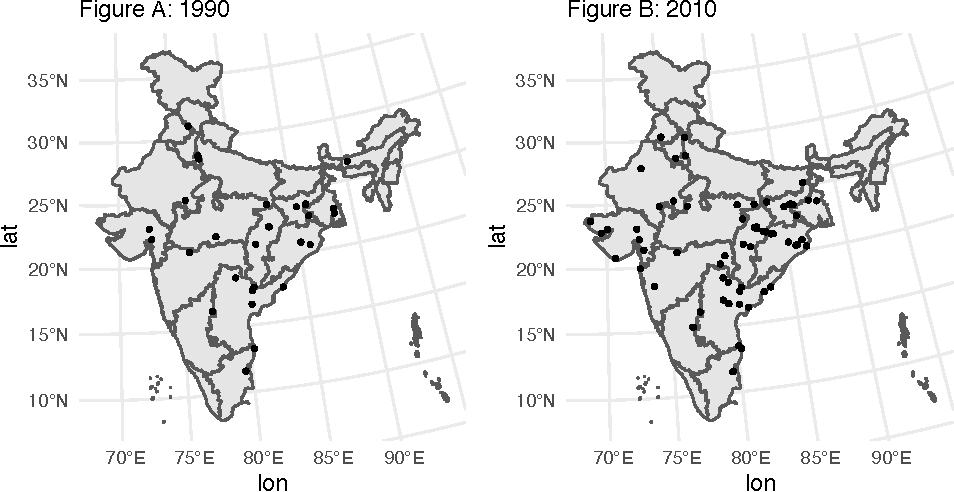
\includegraphics{draft_files/figure-latex/plants-1} \caption[Coal plants in India from 1990 to 2010]{Coal plants in India from 1990 to 2010}\label{fig:plants}\floatfoot*{Note: The top figure shows the location of coal plants in 1990. The bottom figure shows the location of coal plants in 2010.}
\end{figure}

Figure \ref{fig:plants} displays the location of coal plants in India for two specific years: 1990 and 2010. There is a clear increase in the prevalence of coal plants across the country over the two decades. Additionally, the overall capacity from coal plants increased from 42.4 gigawatts to 100.4 gigawatts, an increase of 136.6 percent in just 20 years. This increase is driven both by the roll out of new plants as well as the construction of new units at existing plants, the latter of which is not shown in Figure \ref{fig:plants}.

The second dataset includes agricultural productivity for both the monsoon and winter seasons, from 2002 to 2018. To match other data, I only use the data up to 2013. This data comes from Gangopadhyay et al. (2022) and estimates land productivity (i.e.~yield, in tons per hectare) for the major crops in India, using satellite-derived data. While there is a wealth of literature on measurement error in land (Desiere and Jolliffe 2018; Abay et al. 2022), the authors use a static cropland mask for the productivity estimates. This means that any measurement error will be constant across time and subsumed by the village fixed effects. While the measure of output is also noisy, the use of satellite-derived data and a static cropland mask reduces concerns about measurement error being responsible for the results below. The authors define the monsoon season as June to October and the winter season as November to March. I keep these definitions when matching across data below. This data is also publicly available from Nature's data-sharing website.\footnote{springernature.figshare.com} Since the main regressions below use village fixed effects, any differences in cropping patterns across areas should not bias estimates on changes, as long as these patterns do not change markedly in response to pollution.

The agricultural productivity data is available as raster files with a resolution of 500m. To aggregate this data up to a useful administrative unit, I use village-level shapefiles provided by Asher et al. (2021) and publicly available on the SHRUG platform.\footnote{www.devdatalab.org/shrug\_download/} I aggregate the agricultural productivity data to the village level by extracting mean productivity for each feature in the shapefile. I do this separately for each season -- monsoon and winter -- and each year, from 2002 to 2013.

To measure exposure to pollution from coal plants, I first locate all village centroids located within 30km from a coal plant in a given year. I choose 30km due to previous research on the effects of (air) pollution (Aragón and Rud 2016; Bencko and Symon 1977; Li and Gibson 2014). I then calculate the direction from coal plants to all village centroids within that 30km radius. To define exposure, I then pull daily wind direction data from the National Center for Atmospheric Research.\footnote{climatedataguide.ucar.edu/} For each day, I document whether the wind is blowing towards each village centroid.\footnote{I define ``towards'' as within five degrees to help take into account that I am using village centroids, using the x and y components of wind speed.} I then temporally aggregate this daily data depending on the temporal definition of the corresponding outcome. For example, agricultural productivity is defined across five months (e.g.~the monsoon season is from June to October) so I count the total days a given village is exposed to wind blowing from \emph{any} coal plant within 30km during those five months.

\begin{figure}
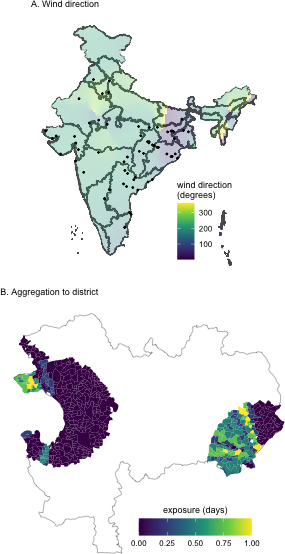
\includegraphics{draft_files/figure-latex/windexample-1} \caption[Wind direction and aggregation examples (2010-01-01)]{Wind direction and aggregation examples (2010-01-01)}\label{fig:windexample}\floatfoot*{Note: The top figure shows the average wind direction on January 1st, 2010, with zero degrees indicating north. The points are the location of coal plants on that date. The bottom figure shows the distribution of pollution exposure in a specific district -- Guna district in Madhya Pradesh -- on the same date.}
\end{figure}

The top panel in Figure \ref{fig:windexample} is an example wind direction raster. The raster shows wind direction for the entirety of India on January 1st, 2010, as well as the location of coal power plants on that date. The prevailing winds on the date differ across the country and, though not shown in the figure, across days. This means that the overall exposure for a given area to coal plant emissions changes across time. I also pull data on particulate matter to help validate this proxy for exposure. This data comes from Hammer et al. (2020) and I also aggregate this to the village using the same method detailed above.

To help understand some of the mechanisms driving the relationship between exposure to emissions and agricultural productivity, I also include household survey data. Unfortunately, I am not aware of any publicly available survey data that covers multiple years and has identifiers below the district level. For example, the ARIS-REDS data\footnote{www.ncaer.org/project/additional-rural-incomes-survey-aris-rural-economic-demographic-survey-reds} includes GPS identifiers for one year, but that only allows GPS matching for a total of two years: 1999 and 2007/2008. The DHS, on the other hand, only has state-level identifiers (except for the newest two waves) and is also not a labor survey. Instead, I use the National Sample Survey (NSS) from the Ministry of Statistics and Programme Implementation.

The NSS is a nationally representative survey that was conducted every couple of years until relatively recently. Many rounds of the NSS also included a module on employment that asked about labor allocation over the previous seven days. I use the 61st, 62nd, 64th, 66th, and 68th rounds of the NSS, all of which include the employment module. The publicly available data also includes the date of survey, which allows me to match pollution exposure to the exact day of the survey.

The biggest issue with using the NSS is that it includes only district-level identifiers. The main exposure variables, on the other hand, are defined at a lower level of aggregation, at the village. I choose to aggregate this village-level exposure to the district level as shown in the second panel of Figure \ref{fig:windexample} -- the district is a randomly selected district in the data, Guna district in Madhya Pradesh. I use the area overlap of the villages with the district to define a weighted average of exposure for the district at a given time. I calculate the area of overlap for each village and the district as well as the overall area of the district and use these variables to define weights for individual villages. Any part of the district that does not overlap with one of the villages -- the white area in Figure \ref{fig:windexample} -- does not have any exposure and, as such, receives a value of zero for exposure.

Finally, I use nightlights as a measure of economic growth (Henderson, Storeygard, and Weil 2012). I also take this data directly from SHRUG and Asher et al. (2021). This covers 1992 through 2013. Some of the older data may not be ideal (Gibson et al. 2021), but this is the only way to document changes in economic growth at a more disaggregated level and at a regular basis. Although satellite imagery is an attractive alternative (Burke et al. 2021), high-resolution satellite imagery does not go back to the early 1990s.

\hypertarget{identification}{%
\subsection{Identification}\label{identification}}

\label{identification}

To calculate the effects of exposure to pollution on different outcomes, I rely on fixed effects and the differential exposure driven by plausibly exogenous wind direction, conditional on total rainfall and average temperature. The regression is of the form \begin{gather} y_{it} = \alpha_{i} + \gamma_{t} + \beta wind_{it} + \delta rain_{it} + \psi temp_{it} + \varepsilon_{it}, \end{gather} where \(y_{it}\) is outcome \(y\) for unit \(i\) at time \(t\), \(\alpha\) is a geographic fixed effects, \(\gamma_t\) is time fixed effects, \(wind_{it}\) is exposure to pollution -- defined using wind direction -- \(rain_{it}\) is total rainfall during the season, and \(temp_{it}\) is average temperature during the season. Although I use \(i\) and \(t\) as subscripts for the fixed effects, note that these change depending on the unit of analysis and the outcome. I explicitly state the level of fixed effects in the tables and results below.

Identification relies on changes in wind direction across time for the same geographic units. In other words, conditional on the fixed effects and weather, I assume changes in wind direction are as good as random and uncorrelated with the outcome -- e.g.~agricultural productivity -- except through exposure to pollution. One major threat to identification is that the building of a coal plant could lead to a spurious correlation between the exposure variable and the outcome. Specifically, since exposure is defined as zero prior to the building of a coal plant, the exposure variable itself might be endogenous even though wind direction is not. To help allay these concerns, I estimate additional regressions restricting the sample to only time periods after which a given location has a coal plant. I also present results using leads to show that future wind direction does not seem to predict current outcomes.

The inclusion of rainfall and temperature is meant to reduce concerns that wind direction may not affect agricultural productivity but, instead, be correlated with it through changes in weather. For example, prevailing winds from one direction may be associated with dry weather, while winds from another direction may be more likely to carry moisture and rain. It is not a priori clear how this would bias the estimates with respect to pollution and coal plants, however. The differences in weather patterns is very context specific and can differ even for villages located near one another. Nonetheless, adding rainfall and temperature should alleviate some of these concerns.

A large question looms with respect to identification: what are the characteristics of areas near the construction of new coal plants? While I examine the identifying assumptions in a panel context below, I begin with this static question here. Table \ref{tab:plantresultstable} presents four separate regressions. The first two columns use 1991 census data -- downloaded from SHRUG -- and the second two columns use 2001 census data, all at the village level. The first column presents results from regressing a dummy for whether there is a coal plant within 30km in 1991 on several census variables. Villages with higher populations and higher literacy in 1991 are more likely to be near a coal plant at the time. Interestingly, however, they are less likely to have a paved road.

\begin{table}

\caption{\label{tab:plantresultstable}Local characteristics and the construction of coal plants}
\centering
\begin{threeparttable}
\begin{tabular}[t]{>{\raggedright\arraybackslash}p{3cm}>{\centering\arraybackslash}p{2cm}>{\centering\arraybackslash}p{2cm}>{\centering\arraybackslash}p{2cm}>{\centering\arraybackslash}p{2cm}}
\toprule
\multicolumn{1}{c}{ } & \multicolumn{2}{c}{1991 census} & \multicolumn{2}{c}{2001 census} \\
\cmidrule(l{3pt}r{3pt}){2-3} \cmidrule(l{3pt}r{3pt}){4-5}
  & 1991 & 2001 & 2001 & 2011\\
\midrule
pop (log) & 0.068*** & 0.0003 & 0.009*** & 0.002***\\
 & (0.0002) & (0.0002) & (0.0003) & (0.0002)\\
literacy (prop) & 0.127*** & -0.005*** & 0.043*** & 0.030***\\
 & (0.002) & (0.001) & (0.002) & (0.002)\\
has paved road & -0.036*** & 0.003*** & -0.008*** & -2.68e-7\\
 & (0.0008) & (0.0004) & (0.0008) & (0.0006)\\
ag productivity &  &  & 0.033*** & 0.005***\\
 &  &  & (0.0005) & (0.0004)\\
sub-sample & all & no plant & all & no plant\\
\midrule
observations & 490,882 & 447,288 & 516,798 & 476,517\\
\bottomrule
\end{tabular}
\begin{tablenotes}[para]
\item Note: Robust standard errors are in parentheses. The outcome in the first column is whether the village is within 30km of a coal plant in 1991. The second column is whether a village in 1991 will have a coal plant in 2001, conditional on not having one in 1991. The last two columns are similarly defined, except using 2001 and 2011 as the years. * p<0.10 ** p<0.05 *** p<0.01
\end{tablenotes}
\end{threeparttable}
\end{table}

The second column keeps the 1991 census data but changes the outcome variable to a dummy for whether there \emph{will be} a coal plant constructed within 30km before 2001. This column restricts the sample to only villages that do not already have a coal plant within 30km in 1991. Population is no longer a significant predictor while the coefficients on literacy and the presence of a paved road have flipped.

The last two columns are particularly relevant to the current results. They present similar results to those in the first two columns, but use the 2001 census data and a dummy for the presence of a coal plant in 2001 and 2011 in columns three and four, respectively. Importantly, I include agricultural productivity in the monsoon season of 2002 -- the earliest year available -- as an additional predictor. In 2001, agricultural productivity is a strong predictor for the presence of a coal plant. Moreover, it is also a significant predictor of the construction of a coal plant between 2001 and 2011 (column four). Given that the coefficient is positive, this indicates that coal plants are more likely to be built in areas with higher agricultural productivity. In other words, any selection in the overall location of coal plants would bias against finding negative effects of pollution on agricultural productivity. However, note that this is not the same as looking at wind direction, though comparing the OLS and IV results below leads to the same conclusion regarding selection.

It is worth taking the time to validate the use of wind direction as a measure of exposure to pollution. Consider the data used for the regressions presented in Table \ref{tab:pollutiontable}. The outcome variable is particulate matter -- specifically, \(\mathrm{PM_{2.5}}\), which is particulate matter no larger than 2.5 micrometers in diameter -- which comes from Hammer et al. (2020). \(\mathrm{PM_{2.5}}\) is one of the harmful byproducts from coal plants, along with sulfur dioxide, different types of nitrogen oxides, and mercury.\footnote{www.epa.gov/airmarkets/power-plants-and-neighboring-communities} This data is available at the monthly level, so in Table \ref{tab:pollutiontable}, I aggregate wind exposure to the monthly level, as well.

\begin{table}

\caption{\label{tab:pollutiontable}Wind direction and particulate matter}
\centering
\begin{threeparttable}
\begin{tabular}[t]{>{\raggedright\arraybackslash}p{4cm}>{\centering\arraybackslash}p{2cm}>{\centering\arraybackslash}p{2cm}>{\centering\arraybackslash}p{2cm}>{\centering\arraybackslash}p{2cm}}
\toprule
\multicolumn{1}{c}{ } & \multicolumn{2}{c}{1998-2015} & \multicolumn{2}{c}{2002-2013} \\
\cmidrule(l{3pt}r{3pt}){2-3} \cmidrule(l{3pt}r{3pt}){4-5}
  & (1) & (2) & (3) & (4)\\
\midrule
wind & 0.045*** & 0.014*** & 0.063*** & 0.015***\\
 & (0.004) & (0.001) & (0.005) & (0.002)\\
\textbf{fixed effects:} & \textbf{} & \textbf{} & \textbf{} & \textbf{}\\
village & Yes & Yes & Yes & Yes\\
month & Yes & No & Yes & No\\
district-month & No & Yes & No & Yes\\
\midrule
observations & 22,345,092 & 22,345,092 & 14,896,728 & 14,896,728\\
\bottomrule
\end{tabular}
\begin{tablenotes}[para]
\item Note: Standard errors are in parentheses and are clustered at the village level. * p<0.10 ** p<0.05 *** p<0.01
\end{tablenotes}
\end{threeparttable}
\end{table}

Both the particulate matter data and the wind data is at the village level, which means the regressions in Table \ref{tab:pollutiontable} are at the village level. As such, the geographic fixed effects are village fixed effects and the temporal fixed effects are month fixed effects. Since the exposure variable is at the village level and we follow villages over time, the standard errors are also clustered at the village level. In columns two and four, I switch the month fixed effects for district-month fixed effects, which considers only villages in the same district in the same month.

In addition to serving as an example, Table \ref{tab:pollutiontable} also helps validate the use of wind direction as a proxy for exposure to pollution. The first two columns include all available years of data while the last two columns restrict estimation only to the years for which the agricultural productivity regressions are estimated. Across all four columns, the story is the same: when the wind is blowing in the direction of a village from a coal plant within 30 kilometers, estimated \(\mathrm{PM_{2.5}}\) is substantially higher. The regressions indicate that one additional day of wind in the direction of the village increases mean \(\mathrm{PM_{2.5}}\) for the month by between 0.01 and 0.06 \(\mathrm{\mu g/m^3}\).

To put these numbers into perspective, the World Health Organization's updated guidelines are that average annual exposure should not exceed 15 \(\mathrm{\mu g/m^3}\). For the month, an increase at the midpoint of the estimated range is equal to an increase of 0.2 percent of the maximum recommended mean concentration from the WHO. This is just a single day of wind in the direction of a village. Since this includes all villages located within 30km of a coal plant, this is evidence that wind direction can have serious repercussions on the health of hundreds of millions of people in India.

\hypertarget{results}{%
\section{Results}\label{results}}

\label{results}

This section presents the main results of this paper. I present three sets of results: one set looking at agricultural productivity, another looking at labor allocation, and a final set looking at nightlights, which are a proxy for economic development. I go through each of these in turn.

\hypertarget{agricultural-productivity}{%
\subsection{Agricultural productivity}\label{agricultural-productivity}}

I first present results for agricultural productivity. The outcome of all the regressions in this section is the log of agricultural land productivity, which is defined as tons per hectare. The first set of results are in Table \ref{tab:yieldtable}. The unit of analysis is the vilalge-year-season -- from 2002 to 2013 -- the geographic fixed effect is the village-season, and the temporal fixed effect is the year. The exposure variable is defined for the entire season. Since Gangopadhyay et al. (2022) define both the monsoon (kharif) season and the winter (rabi) season as five months long, I do as well, using the same five months as the authors. This implies that the exposure variable ranges from zero to slightly more than 150.

The first column presents the most simple results, with only the wind exposure variable and the fixed effects. The second column adds a rainfall -- defined as the total rainfall in the season -- and average temperature variable, the addition of which is motivated by the fact that changes in wind direction could be correlated with changes in weather. However, the coefficient on the wind exposure variable is completely unchanged by the addition of the two weather variables, indicating that weather may not be as worrisome of a confounder as thought. The direction of the weather coefficients is also consistent with expectations; higher rainfall is good for agricultural productivity while higher temperature is not.

Column three adds district-by-year-by-season fixed effects as an additional robustness checks. This addition decreases the magnitude of the exposure variable but it remains negative and significant. However, part of this may be due to the fact that the new fixed effects soak up much of the variation in the exposure variable, as shown in Figure \ref{fig:windexample}. The last two columns separate the effects into the monsoon season and the winter season, but the overall effect is roughly similar, though rainfall has a larger effect in the monsoon season than the winter season, which is unsurprising given the winter season is driven by irrigation in many areas.

\begin{table}

\caption{\label{tab:yieldtable}Wind direction and agricultural productivity}
\centering
\begin{threeparttable}
\begin{tabular}[t]{>{\raggedright\arraybackslash}p{3cm}>{\centering\arraybackslash}p{2cm}>{\centering\arraybackslash}p{2cm}>{\centering\arraybackslash}p{2cm}>{\centering\arraybackslash}p{2cm}>{\centering\arraybackslash}p{2cm}}
\toprule
\multicolumn{1}{c}{ } & \multicolumn{3}{c}{all} & \multicolumn{1}{c}{monsoon} & \multicolumn{1}{c}{winter} \\
\cmidrule(l{3pt}r{3pt}){2-4} \cmidrule(l{3pt}r{3pt}){5-5} \cmidrule(l{3pt}r{3pt}){6-6}
  & (1) & (2) & (3) & (4) & (5)\\
\midrule
wind & -0.003*** & -0.003*** & -0.0007*** & -0.002*** & -0.004***\\
 & (0.0002) & (0.0002) & (9.24e-5) & (0.0002) & (0.0003)\\
rain (z) &  & 0.029*** & 0.008*** & 0.075*** & 0.006***\\
 &  & (0.0004) & (0.001) & (0.002) & (0.0005)\\
mean temp (10s) &  & -0.0004*** & -0.007*** & -0.002*** & -0.008***\\
 &  & (5.53e-5) & (0.0004) & (0.0001) & (9.83e-5)\\
\textbf{fixed effects:} & \textbf{} & \textbf{} & \textbf{} & \textbf{} & \textbf{}\\
village-season & Yes & Yes & Yes & No & No\\
year & Yes & Yes & No & Yes & Yes\\
district-year-season & No & No & Yes & No & No\\
village & No & No & No & Yes & Yes\\
\midrule
observations & 2,387,417 & 2,371,221 & 2,371,221 & 1,256,951 & 1,114,270\\
\bottomrule
\end{tabular}
\begin{tablenotes}[para]
\item Note: Standard errors are in parentheses and are clustered at the village level. The outcome in all regressions is estimated agricultural yield, defined as tons per hectare. * p<0.10 ** p<0.05 *** p<0.01
\end{tablenotes}
\end{threeparttable}
\end{table}

To put the size of the coefficient in context, it is worth digging a little deeper into the exposure variable. The mean within-village absolute deviation in wind exposure is approximately 8.06 days, meaning that the average change in agricultural productivity from year-to-year due to nothing but changes in wind patterns carrying particulate matter is around 2.4 percent relative to the mean. This implies that swings in agricultural productivity -- due to wind direction -- of more than five percent are probably quite common, since the absolute deviation includes deviations below and above the mean.

\begin{table}

\caption{\label{tab:yieldtablepm}Particulate matter (PM 2.5) and agricultural productivity}
\centering
\begin{threeparttable}
\begin{tabular}[t]{>{\raggedright\arraybackslash}p{3cm}>{\centering\arraybackslash}p{2cm}>{\centering\arraybackslash}p{2cm}>{\centering\arraybackslash}p{2cm}>{\centering\arraybackslash}p{2cm}>{\centering\arraybackslash}p{2cm}}
\toprule
\multicolumn{1}{c}{ } & \multicolumn{3}{c}{all} & \multicolumn{1}{c}{monsoon} & \multicolumn{1}{c}{winter} \\
\cmidrule(l{3pt}r{3pt}){2-4} \cmidrule(l{3pt}r{3pt}){5-5} \cmidrule(l{3pt}r{3pt}){6-6}
  & (1) & (2) & (3) & (4) & (5)\\
\midrule
particulate matter & 0.0000 & 0.0005*** & -0.0004*** & 0.002*** & 0.0004***\\
(PM 2.5, '000s) & (0.0000) & (3.17e-5) & (5.72e-5) & (9.87e-5) & (3.7e-5)\\
rain (z) &  & 0.030*** & 0.008*** & 0.075*** & 0.007***\\
 &  & (0.0004) & (0.001) & (0.002) & (0.0005)\\
mean temp (10s) &  & -0.0003*** & -0.007*** & -0.002*** & -0.008***\\
 &  & (5.63e-5) & (0.0004) & (0.0001) & (9.79e-5)\\
\textbf{fixed effects:} & \textbf{} & \textbf{} & \textbf{} & \textbf{} & \textbf{}\\
village-season & Yes & Yes & Yes & No & No\\
year & Yes & Yes & No & Yes & Yes\\
district-year-season & No & No & Yes & No & No\\
village & No & No & No & Yes & Yes\\
\midrule
observations & 2,387,417 & 2,371,221 & 2,371,221 & 1,256,951 & 1,114,270\\
\bottomrule
\end{tabular}
\begin{tablenotes}[para]
\item Note: Standard errors are in parentheses and are clustered at the village level. The outcome in all regressions is estimated agricultural yield, defined as tons per hectare. * p<0.10 ** p<0.05 *** p<0.01
\end{tablenotes}
\end{threeparttable}
\end{table}

Of course, it is not wind, per se, that we are interested in. Instead, we are actually interested in better understanding the effects of exposure to pollution on agricultural productivity. Table \ref{tab:yieldtablepm} presents the same regressions as Table \ref{fig:yieldtable}, with a key difference: instead of wind exposure, it uses average concentration of \(\mathrm{PM_{2.5}}\) -- from Hammer et al. (2020) -- during the season as the key explanatory variable. I rescale particulate matter by dividing by one thousand to help with presentation of the coefficients. Several interesting patterns emerge. In the first column we see no relationship between particulate matter and agricultural productivity, while there is actually a positive relationship in columns two, four, and five. There is a small, negative relationship between pollution and productivity in column three.

Recall, however, the results from above: coal plants were placed in places with higher average agricultural productivity. This means that the simple regressions in \ref{tab:yieldtablepm} might actually be biased upwards: although pollution might negatively affect productivity, pollution is higher in more productive areas due to the endogenous placement of coal plants in the study areas. To recover the actual effect of pollution, we need an instrument. If, conditional on the fixed effects and weather variables, wind direction is exogenous and only affects agricultural productivity through pollution -- which seems reasonable since it is hard to imagine what other variables it might affect -- then it is a valid instrument for pollution.

I present the IV results in Table \ref{tab:yieldtabletwo}, with the second-stage results in the top panel and the first-stage results in the bottom panel. The first-stage results make clear how strong of an instrument wind is; the t-statistic in column one, for example, is almost 48 while it is still well above 10 in column three, which translates to a first-stage F-statistic of 195, meeting even the higher bar for the first-stage F-test argued for by D. S. Lee et al. (2022). Also note that the coefficients are quite different from those in Table \ref{tab:pollutiontable} because the unit of analysis in Table \ref{tab:yieldtabletwo} is the season, while in Table \ref{tab:pollutiontable} the unit of analysis is the month.

The second-stage results first indicate that \(\mathrm{PM_{2.5}}\) is a very strong predictor of agricultural productivity. The smallest coefficient -- that for the monsoon season in column (4) -- and the mean absolute deviation for \(\mathrm{PM_{2.5}}\) point to a change in agricultural productivity of around 23 percent, which is much higher than the wind results documented above. This makes sense, of course, since the IV is essentially scaling up the effects of wind. The comparison of the results to those in the previous table also confirm the concerns around endogenous placement of coal plants. The coefficients in Table \ref{tab:yieldtabletwo} are always more negative than those in Table \ref{tab:yieldtablepm}, and sometimes substantially so. In other words, the simple regression of agricultural productivity on pollution results in coefficients on pollution that are upwards biased, since coal plants are placed in more productive areas. The IV strategy corrects this bias and leads to a robust, negative relationship between pollution and agricultural productivity.

\begin{table}

\caption{\label{tab:yieldtabletwo}Pollution and agricultural productivity, IV estimates}
\centering
\begin{threeparttable}
\begin{tabular}[t]{>{\raggedright\arraybackslash}p{3cm}>{\centering\arraybackslash}p{2cm}>{\centering\arraybackslash}p{2cm}>{\centering\arraybackslash}p{2cm}>{\centering\arraybackslash}p{2cm}>{\centering\arraybackslash}p{2cm}}
\toprule
\multicolumn{1}{c}{ } & \multicolumn{3}{c}{all} & \multicolumn{1}{c}{monsoon} & \multicolumn{1}{c}{winter} \\
\cmidrule(l{3pt}r{3pt}){2-4} \cmidrule(l{3pt}r{3pt}){5-5} \cmidrule(l{3pt}r{3pt}){6-6}
  & (1) & (2) & (3) & (4) & (5)\\
\midrule
particulate matter & -0.021*** & -0.024*** & -0.032*** & -0.012*** & -0.035***\\
(PM 2.5) & (0.001) & (0.002) & (0.005) & (0.001) & (0.003)\\
rain (z) &  & -0.011*** & -4.24e-5 & 0.078*** & -0.042***\\
 &  & (0.003) & (0.002) & (0.002) & (0.004)\\
mean temp (10s) &  & -0.005*** & -0.007*** & -0.002*** & -0.008***\\
 &  & (0.0003) & (0.0004) & (0.0001) & (0.0001)\\
\textbf{fixed effects:} & \textbf{} & \textbf{} & \textbf{} & \textbf{} & \textbf{}\\
village-season & Yes & Yes & Yes & No & No\\
year & Yes & Yes & No & Yes & Yes\\
district-year-season & No & No & Yes & No & No\\
village & No & No & No & Yes & Yes\\
\midrule
observations & 2,387,417 & 2,371,221 & 2,371,221 & 1,256,951 & 1,114,270\\
\midrule
\textbf{first stage:} & \textbf{} & \textbf{} & \textbf{} & \textbf{} & \textbf{}\\
wind & 0.145*** & 0.111*** & 0.022*** & 0.157*** & 0.105***\\
 & (0.002) & (0.002) & (0.002) & (0.002) & (0.004)\\
rain (z) &  & -1.68*** & -0.239*** & 0.225*** & -1.37***\\
 &  & (0.011) & (0.017) & (0.015) & (0.010)\\
mean temp (10s) &  & -0.192*** & 0.002 & -0.021*** & -0.007***\\
 &  & (0.0009) & (0.004) & (0.001) & (0.002)\\
\bottomrule
\end{tabular}
\begin{tablenotes}[para]
\item Note: Standard errors are in parentheses and are clustered at the village level. The outcome in all regressions is estimated agricultural yield, defined as tons per hectare. * p<0.10 ** p<0.05 *** p<0.01
\end{tablenotes}
\end{threeparttable}
\end{table}

Having established that exposure to pollution has a negative effect on agricultural productivity, I now move to heterogeneity in these effects. Table \ref{tab:yieldtablehet} presents four different analyses: effects of exposure by maximum exposure, multiplicative effects of shocks, the possibility of non-linearities, and the differential effects of exposure based on initial agricultural productivity.

The first two columns split the sample based on maximum exposure; villages with maximum exposure above the median are included in column (1) while those below the median are in column (2). Interestingly, the largest effects are seen on villages in the lower half of the distribution. Apparently, smaller maximum effects lead to larger overall effects of pollution exposure on agricultural productivity. In other words, it is not the places where wind is most likely to blow from a coal plant that experience the largest decrease in productivity in response to an additional day of wind-driven pollution.

\begin{table}

\caption{\label{tab:yieldtablehet}Heterogeneity in the effects of pollution on productivity}
\centering
\begin{threeparttable}
\begin{tabular}[t]{>{\raggedright\arraybackslash}p{3cm}>{\centering\arraybackslash}p{2cm}>{\centering\arraybackslash}p{2cm}>{\centering\arraybackslash}p{2cm}>{\centering\arraybackslash}p{2cm}>{\centering\arraybackslash}p{2cm}}
\toprule
\multicolumn{1}{c}{ } & \multicolumn{1}{c}{>p(50)} & \multicolumn{1}{c}{<=p(50)} & \multicolumn{3}{c}{all} \\
\cmidrule(l{3pt}r{3pt}){2-2} \cmidrule(l{3pt}r{3pt}){3-3} \cmidrule(l{3pt}r{3pt}){4-6}
  & (1) & (2) & (3) & (4) & (5)\\
\midrule
wind & -0.003*** & -0.033*** & -0.004*** & 0.0006 & 0.000\\
 & (0.0002) & (0.002) & (0.0003) & (0.0005) & (0.001)\\
rain (z) & 0.028*** & 0.032*** & 0.028*** & 0.028*** & 0.028***\\
 & (0.0006) & (0.0005) & (0.0004) & (0.0004) & (0.0004)\\
mean temp (10s) & -0.001*** & 0.0006*** & -0.0004*** & -0.0004*** & -0.0004***\\
 & (7.66e-5) & (7.9e-5) & (5.55e-5) & (5.56e-5) & (5.49e-5)\\
wind x rain &  &  & 0.0005*** &  & \\
 &  &  & (6.74e-5) &  & \\
wind squared &  &  &  & -0.0002*** & \\
 &  &  &  & (3.58e-5) & \\
wind x starting yield &  &  &  &  & -0.001**\\
 &  &  &  &  & (0.0006)\\
\textbf{fixed effects:} & \textbf{} & \textbf{} & \textbf{} & \textbf{} & \textbf{}\\
village-season & Yes & Yes & Yes & Yes & Yes\\
year & Yes & Yes & Yes & Yes & Yes\\
\midrule
observations & 1,112,082 & 1,259,139 & 2,371,221 & 2,371,221 & 2,367,248\\
\bottomrule
\end{tabular}
\begin{tablenotes}[para]
\item Note: Standard errors are in parentheses and are clustered at the village level. The outcome in all regressions is estimated agricultural yield, defined as tons per hectare. The first two columns split the sample based on the *maximum* observed exposure. * p<0.10 ** p<0.05 *** p<0.01
\end{tablenotes}
\end{threeparttable}
\end{table}

Column three looks add the possible multiplicative effects of rainfall shocks and pollution shocks on agricultural productivity. In previous tables, rainfall always entered the regression positively -- as we would expect -- indicating that higher rainfall in a given season leads to higher agricultural productivity. However, an interesting question is whether rainfall and pollution shocks might interact. The positive coefficient on the interaction term between days of wind and rainfall during the agricultural season indicates that there is a multiplicative effect of shocks; when wind days are higher (bad) and rainfall is lower (bad), the overall negative effects are even worse than when just one shock happens. Considering that climate change is leading to more variable rainfall and more negative rainfall shocks, these results are potentially worrisome, especially for smallholders.

Column four adds a quadratic in wind to see if the negative effects of pollution on agricultural productivity are increase or decreasing in wind. In column four, the coefficient on the linear term is 0.0006 while the coefficient on the quadratic term is -0.0002, meaning that the effect of wind is decreasing for any days of wind over three The negative coefficient also indicates that this negative effect is consistently decreasing, meaning the effect gets worse as average wind days gets higher. Note that this is somewhat different from the regressions in the first two columns, which split the sample by the \emph{maximum} days of wind observed in the sample, not the mean.

In the final column I add to the regression an interaction between wind and initial agricultural productivity (defined in 2002, the first year observed in the productivity data). The linear term drops out of the regression since it is invariant within villages, leaving just the interaction term. The negative coefficient on the interaction term of -0.001 indicates that the effect of pollution is more negative in areas where agricultural productivity is higher. Note that agricultural productivity is defined in logs, so this can be interpreted as a percentage effect, not a level effect. Apparently, wind-driven pollution is particularly detrimental to agricultural productivity in the most productive places.

\hypertarget{robustness-checks}{%
\subsection{Robustness checks}\label{robustness-checks}}

I present two separate robustness checks in the appendix. The first set of analyses attempts to separate the possible endogenous location of coal plants from outcomes. Specifically, prior to the opening of a new coal plant in an area, all villages receive a zero for wind. This means that, even if wind direction is exogenous, the opening of the coal plant could lead to correlations between the error term and the wind variable.

Although the results with district-year-season help mitigate this concern, Table \ref{tab:yieldtablepostplant} in the appendix checks this possibility in a different way. Specifically, I restrict the sample to only village-years \emph{after} the introduction of a coal plant. This drops any pre-plant-opening observations -- all of which are mechanically zeros for wind -- to prevent endogeneity due to the opening. The coefficients in Table \ref{tab:yieldtablepostplant} show that the overall effects are essentially unchanged, with just a small change in coefficient magnitude (driven mostly by rounding).

The second robustness check includes leads for wind to see if they predict current year productivity. I present these results in \ref{tab:yieldtableleads}. The second column includes district-year-season fixed effects, while the first does not. The results make clear the importance of including trends or district-year fixed effects. In the first column, leads seem to predict productivity. However, this relationship disappears in the second column, indicating that the previous results with district-year fixed effects are likely the most reliable.

\hypertarget{labor-allocation}{%
\subsection{Labor allocation}\label{labor-allocation}}

The previous set of results show a consistent negative effect of wind-driven pollution on agricultural productivity. A key question is the mechanism through which this happens; is this driven by changes in labor allocation/productivity or by changes in land productivity? While I cannot definitely prove the mechanism, I can shed some light on possibilities by looking at labor allocation decisions. Since these shocks generally happen after initial planting decisions, it seems unlikely that changes in land \emph{allocation} could drive the results.

Table \ref{tab:labortable} presents results for labor allocation over the last seven days using the National Sample Survey and the methodology described above. Since the labor recall is for seven days, labor allocation ranges from zero to seven, as does the wind variable. Recall that the data is at the district level, not the village level. However, it is also more temporally disaggregated, with rolling interviews throughout the year-long survey. Figure \ref{fig:laborplot} in the appendix shows this temporal distribution across the five waves of the survey. Since I can no longer include district-by-month fixed effects, I instead opt for district-level trends to help take into account aggregate temporal changes in outcomes.

\begin{table}

\caption{\label{tab:labortablerural}Wind direction and labor allocation, rural only}
\centering
\begin{threeparttable}
\begin{tabular}[t]{>{\raggedright\arraybackslash}p{3cm}>{\centering\arraybackslash}p{1.5cm}>{\centering\arraybackslash}p{1.5cm}>{\centering\arraybackslash}p{1.5cm}>{\centering\arraybackslash}p{1.5cm}>{\centering\arraybackslash}p{1.5cm}>{\centering\arraybackslash}p{1.5cm}}
\toprule
  & all & all & self & wage & farm & non-farm\\
\midrule
\textbf{rural} & \textbf{} & \textbf{} & \textbf{} & \textbf{} & \textbf{} & \textbf{}\\
wind & -0.112*** & -0.118*** & -0.050* & -0.068** & -0.002 & -0.116***\\
 & (0.036) & (0.029) & (0.030) & (0.031) & (0.028) & (0.034)\\
DV mean & 3.499 & 3.499 & 2.172 & 1.327 & 1.260 & 2.240\\
observations & 529,562 & 529,466 & 529,466 & 529,466 & 529,466 & 529,466\\
\midrule
\textbf{urban} & \textbf{} & \textbf{} & \textbf{} & \textbf{} & \textbf{} & \textbf{}\\
wind & -0.020 & -0.030 & -0.011 & -0.019 & 0.023* & -0.053\\
 & (0.033) & (0.041) & (0.039) & (0.031) & (0.014) & (0.048)\\
DV mean & 3.040 & 3.040 & 1.393 & 1.647 & 0.101 & 2.939\\
observations & 369,483 & 369,390 & 369,390 & 369,390 & 369,390 & 369,390\\
\midrule
controls & No & Yes & Yes & Yes & Yes & Yes\\
\textbf{fixed effects:} & \textbf{} & \textbf{} & \textbf{} & \textbf{} & \textbf{} & \textbf{}\\
district & Yes & Yes & Yes & Yes & Yes & Yes\\
state-month & Yes & Yes & Yes & Yes & Yes & Yes\\
\bottomrule
\end{tabular}
\begin{tablenotes}[para]
\item Note: Standard errors are in parentheses and are clustered at the district level. Control variables include female, age, age squared, and (years of) education. The outcome in each regression is days worked in the previous seven days. * p<0.10 ** p<0.05 *** p<0.01
\end{tablenotes}
\end{threeparttable}
\end{table}

There are some interesting results in Table \ref{tab:labortable}. The first two columns show a marginally significant decrease in overall labor allocation (where ``labor'' is defined as non-domestic self and wage employment). The third and fourth columns show that this overall decrease is predominantly from wage employment, not self employment. An additional day of wind over the last seven decreases wage employment by 0.034 days in the district. Mean wage employment is 1.458 days, meaning one day of wind decreases wage employment by 2.3 percent of the mean. Since much of the district is not covered by ``treated'' villages, this is actually a rather substantive effect on the villages involved.

The last two columns split the effects by sector, into farm and non-farm employment. Although agricultural (land) productivity decreases when wind blows in the direction of villages, overall labor allocation to farm labor actually goes \emph{up}, by around 4.5 percent of the mean of 0.784 days. Non-farm labor, on the other hand, goes down, by around 2.4 percent of the mean of 2.527 days.

There are two possible explanations for this pattern of results. First, it could be that land productivity goes down, leading farmers to increase their farm labor allocation in an attempt to compensate for the decreased productivity. A second possibility is that pollution does not affect land productivity at all, at least not directly. In this scenario, the worsening air quality could lead to decreased labor productivity, meaning that ``effective labor'' essentially decreases when pollution is higher.

Table \ref{tab:labortablemonsoon} and Table \ref{tab:labortablewinter} in the appendix disaggregate these effects into the monsoon and winter seasons. Apparently, the entirety of the effect is driven by changes in labor allocation during the monsoon season. The dynamics across seasons apparently lead to large differences in the effects of pollution on labor allocation.

One way to provide suggestive evidence of mechanisms is to explore heterogeneity in the effects. Previous research has shown larger effects of pollution on the health of the oldest (Deryugina et al. 2019). The labor sample includes all adults between 15 and 60 years of age. To look at heterogeneity by age, I present an additional set of results interacting the wind variable with an indicator for whether an individual is over 37 years of age.\footnote{This splits the sample into two equal bins of age: those who are 15-37 and those who are 38-60.} These results are in Table \ref{tab:labortableold}, which otherwise presents the same specifications in the last five columns as \ref{tab:labortable}.

Table \ref{tab:labortableold} presents a very clear set of results: the effects are always larger (more negative) for older adults. Particularly interestingly, we now see that the mean-zero effect on self employment in the previous table is driven by two stark contrasts: a large increase for the younger group and a large decrease for the older group. For the youngest group, this increase appears in farm labor, indicating likely increases in farm self-employment. The oldest, on the other hand, have large decreases in both farm and non-farm labor, with larger decreases in the latter.

To put some of these changes in context, an additional day of exposure to pollution from wind increases self-employment for the younger half of the sample by around six percent of the mean and increases farm employment for the younger half by almost 10 percent of the mean. For the older half, on the other hand, an additional day of exposure decreases self-employment and non-farm employment by around five percent of their means.

While speculative, one possible explanation for this pattern is a decrease in labor productivity. While the youngest may be able to readjust and increase their overall self-employment labor allocation, perhaps the oldest cannot due to, for example, health effects of pollution, which are well documented (Bentayeb et al. 2012; Pope III 2000).\footnote{Much of the literature also suggests the youngest are at significant risk of mortality and morbidities. However, given my focus on labor allocation, I only discuss older adults here.} We see decreases in overall agricultural productivity, despite an increase in overall farm labor. We also see decreases in non-farm employment, indicating that individuals are reallocating labor from the non-farm sector to the farm sector.

It is worth noting that the larger negative effects for older adults is more consistent with a labor story than a land story; it is hard to imagine these patterns emerging if the only effects were through land productivity changes. The overall decrease in non-farm employment is more compatible with a labor health/productivity story, though with general equilibrium effects in agriculture spillover over into the non-farm sector, this need not necessarily be the case.

In addition, Table \ref{tab:labortableoldstate} in the appendix presents one additional set of results to support a labor story. Changes in land productivity should be relatively fixed in a short period of time. For example, if we focus on just a single month in a single district, the overall effects driven by changes in land productivity should be constant even though pollution may have differential effects throughout the month on labor productivity, which responds more immediately to changes in ar quality. Table \ref{tab:labortableoldstate} changes the specification to include district-by-year-by-month fixed effects. In other words, the results compare people in the same district in the same month, but who may have differential exposure to pollution simply because they were interviewed at a slightly different time.

The overall pattern of results stays the same when we shift the focus. Overall labor allocation increases for the youngest, but decreases for the oldest, and this is driven completely by self employment. There are decreases in both farm and non-farm employment for the oldest, while the youngest show increases in non-farm employment, but not farm employment -- which is a change from the previous results. The overall story remains the same, however, which is further evidence of effects being driven primarily through changes in labor allocation and productivity.

Finally, Table \ref{tab:wagestable} in the appendix shows that there are no significant changes in daily wages, though the overall direction of wage changes would be ambiguous, anyway. While reduced productivity might lead to lower wages, decreased labor supply could also put upward pressure on wages.

\hypertarget{nightlights}{%
\subsection{Nightlights}\label{nightlights}}

Pollution leads to lower agricultural productivity as well as changes in labor allocation. This leads to an obvious question: might higher levels of pollution also directly affect economic growth? To explore this question, I look at changes in nightlights relative to changes in pollution. It seems reasonable to think that pollution might affect nightlights with a lag, so I include the lag of pollution rather than contemporaneous pollution.

\begin{table}

\caption{\label{tab:ntltable}Wind direction and nightlight growth}
\centering
\begin{threeparttable}
\begin{tabular}[t]{>{\raggedright\arraybackslash}p{3cm}>{\centering\arraybackslash}p{2cm}>{\centering\arraybackslash}p{2cm}>{\centering\arraybackslash}p{2cm}>{\centering\arraybackslash}p{2cm}}
\toprule
  & (1) & (2) & (3) & (4)\\
\midrule
wind (lag) & -0.024*** & -0.024*** &  & \\
 & (0.003) & (0.003) &  & \\
wind (lead) &  &  & -0.001 & -0.001\\
 &  &  & (0.002) & (0.002)\\
\textbf{fixed effects:} & \textbf{} & \textbf{} & \textbf{} & \textbf{}\\
village & Yes & Yes & Yes & Yes\\
year & Yes & Yes & Yes & Yes\\
\textbf{varying slopes:} & \textbf{} & \textbf{} & \textbf{} & \textbf{}\\
year (by village) & Yes & Yes & Yes & Yes\\
\midrule
observations & 1,694,535 & 1,694,535 & 1,807,504 & 1,807,504\\
\bottomrule
\end{tabular}
\begin{tablenotes}[para]
\item Note: Standard errors are in parentheses and are clustered at the village level. The outcome in all regressions is logged nightlights. Rainfall is included in columns (2) and (4). * p<0.10 ** p<0.05 *** p<0.01
\end{tablenotes}
\end{threeparttable}
\end{table}

I present these results in Table \ref{tab:ntltable}. To help simplify the coefficients, I recode wind to be the proportion of days in the year that a given village experiences wind in their direction, from a coal plant. Mean wind in this new specification is 0.066, indicating that a village in the sample experiences wind in its direction on around 6.6 percent of days, or 24 days of the year.

We see a strong, negative relationship between pollution (lagged wind) and nightlights. Going from the 25th percentile to the 75th percentile of wind exposure is synonymous with a decrease in the growth of nightlights within a village by around 0.7 percent. While this is a relatively small magnitude, it is worth noting that there are more than 100,000 villages in this sample. While the effect for a single village might be small, the overall, aggregate effect on growth is quite substantial. To put this number in perspective, Castelló-Climent, Chaudhary, and Mukhopadhyay (2018) argue that a standard-deviation increase in the share of adults with a university education leads to 12 percent higher nightlights in India, while Storeygard (2016) shows that a four-fold increase in oil prices over six years leads to seven percent lower nightlights at a distance of around 500km from the nearest large port in sub-Saharan Africa. In other words, the 0.7 percent change in nightlights is quite large given this is annual variation.

\hypertarget{conclusion}{%
\section{Conclusion}\label{conclusion}}

\label{conclusion}

The rapid growth of coal power plants has also led to increases in emissions from the burning of coal. In this paper, I show some of the negative effects associated with this burning: decreased agricultural productivity. I find clear indications that pollution from coal plants leads to lower agricultural productivity. Importantly, I use exogenous changes in wind direction to measure exposure to pollution and show that these effects are robust to a range of alternative specifications.

Results indicate that these effects may be driven by changes in labor allocation patterns. In addition, the negative labor effects are concentrated in older adults, which is consistent with previous research on the effects of pollution on health in adults. Despite this, I am unable to rule out direct effects on land productivity with the data available.

Finally, these negative effects are also seen in aggregate economic development, with pollution leading to decreases in the growth of nightlights. These effects, though small for an individual village, are quite large in overall terms, indicating that pollution from coal plants can have effects on overall economic development.

These results, of course, do not address possible positive effects of the building of additional power plants, which can lead to increased electricity access. As such, the main conclusion is that the location of new power generation facilities may be particularly important for multiple aspects of economic activity, not just health and mortality.

\FloatBarrier
\newpage
\singlespacing

\hypertarget{references}{%
\section*{References}\label{references}}
\addcontentsline{toc}{section}{References}

\hypertarget{refs}{}
\begin{CSLReferences}{1}{0}
\leavevmode\vadjust pre{\hypertarget{ref-abay2022nonclassical}{}}%
Abay, Kibrom A, Christopher B Barrett, Talip Kilic, Heather Moylan, John Ilukor, and Wilbert Drazi Vundru. 2022. {``{Nonclassical Measurement Error and Farmers? Response to Information Reveal Behavioral Anomalies}.''}

\leavevmode\vadjust pre{\hypertarget{ref-aragon2016polluting}{}}%
Aragón, Fernando M, and Juan Pablo Rud. 2016. {``{Polluting industries and agricultural productivity: Evidence from mining in Ghana}.''} \emph{{The Economic Journal}} 126 (597): 1980--2011.

\leavevmode\vadjust pre{\hypertarget{ref-arceo2016does}{}}%
Arceo, Eva, Rema Hanna, and Paulina Oliva. 2016. {``{Does the effect of pollution on infant mortality differ between developing and developed countries? Evidence from Mexico City}.''} \emph{{The Economic Journal}} 126 (591): 257--80.

\leavevmode\vadjust pre{\hypertarget{ref-almn2021}{}}%
Asher, Sam, Tobias Lunt, Ryu Matsuura, and Paul Novosad. 2021. {``{Development Research at High Geographic Resolution: An Analysis of Night Lights, Firms, and Poverty in India using the SHRUG Open Data Platform}.''} \emph{{The World Bank Economic Review}}.

\leavevmode\vadjust pre{\hypertarget{ref-bencko1977health}{}}%
Bencko, Vladimir, and Karel Symon. 1977. {``Health Aspects of Burning Coal with a High Arsenic Content.''} \emph{{Environmental Research}} 13 (3): 378--85.

\leavevmode\vadjust pre{\hypertarget{ref-bentayeb2012adverse}{}}%
Bentayeb, Malek, Marzia Simoni, Nour Baiz, Dan Norback, Sandra Baldacci, Sara Maio, Giovanni Viegi, Isabella Annesi-Maesano, Geriatric Study in Europe on Health Effects of Air Quality in Nursing Homes (GERIE) Group, et al. 2012. {``Adverse Respiratory Effects of Outdoor Air Pollution in the Elderly.''} \emph{{The International Journal of Tuberculosis and Lung Disease}} 16 (9): 1149--61.

\leavevmode\vadjust pre{\hypertarget{ref-brunekreef2002air}{}}%
Brunekreef, Bert, and Stephen T Holgate. 2002. {``{Air pollution and health}.''} \emph{{The Lancet}} 360 (9341): 1233--42.

\leavevmode\vadjust pre{\hypertarget{ref-burke2021using}{}}%
Burke, Marshall, Anne Driscoll, David B Lobell, and Stefano Ermon. 2021. {``{Using satellite imagery to understand and promote sustainable development}.''} \emph{Science} 371 (6535): eabe8628.

\leavevmode\vadjust pre{\hypertarget{ref-burney2014recent}{}}%
Burney, Jennifer, and V Ramanathan. 2014. {``{Recent climate and air pollution impacts on Indian agriculture}.''} \emph{{Proceedings of the National Academy of Sciences}} 111 (46): 16319--24.

\leavevmode\vadjust pre{\hypertarget{ref-castello2018higher}{}}%
Castelló-Climent, Amparo, Latika Chaudhary, and Abhiroop Mukhopadhyay. 2018. {``{Higher education and prosperity: From Catholic missionaries to luminosity in India}.''} \emph{{The Economic Journal}} 128 (616): 3039--75.

\leavevmode\vadjust pre{\hypertarget{ref-chang2019effect}{}}%
Chang, Tom Y, Joshua Graff Zivin, Tal Gross, and Matthew Neidell. 2019. {``{The effect of pollution on worker productivity: evidence from call center workers in China}.''} \emph{{American Economic Journal: Applied Economics}} 11 (1): 151--72.

\leavevmode\vadjust pre{\hypertarget{ref-chen2022effect}{}}%
Chen, Shuai, Paulina Oliva, and Peng Zhang. 2022. {``{The effect of air pollution on migration: evidence from China}.''} \emph{{Journal of Development Economics}} 156: 102833.

\leavevmode\vadjust pre{\hypertarget{ref-currie2014we}{}}%
Currie, Janet, Joshua Graff Zivin, Jamie Mullins, and Matthew Neidell. 2014. {``{What do we know about short-and long-term effects of early-life exposure to pollution?}''} \emph{{Annual Review Resource Economics}} 6 (1): 217--47.

\leavevmode\vadjust pre{\hypertarget{ref-deryugina2019mortality}{}}%
Deryugina, Tatyana, Garth Heutel, Nolan H Miller, David Molitor, and Julian Reif. 2019. {``{The mortality and medical costs of air pollution: Evidence from changes in wind direction}.''} \emph{{American Economic Review}} 109 (12): 4178--4219.

\leavevmode\vadjust pre{\hypertarget{ref-desiere2018land}{}}%
Desiere, Sam, and Dean Jolliffe. 2018. {``{Land productivity and plot size: Is measurement error driving the inverse relationship?}''} \emph{{Journal of Development Economics}} 130: 84--98.

\leavevmode\vadjust pre{\hypertarget{ref-dinkelman2011effects}{}}%
Dinkelman, Taryn. 2011. {``{The effects of rural electrification on employment: New evidence from South Africa}.''} \emph{{American Economic Review}} 101 (7): 3078--108.

\leavevmode\vadjust pre{\hypertarget{ref-ebenstein2016long}{}}%
Ebenstein, Avraham, Victor Lavy, and Sefi Roth. 2016. {``{The long-run economic consequences of high-stakes examinations: Evidence from transitory variation in pollution}.''} \emph{{American Economic Journal: Applied Economics}} 8 (4): 36--65.

\leavevmode\vadjust pre{\hypertarget{ref-gangopadhyay2022new}{}}%
Gangopadhyay, Prasun K, Paresh B Shirsath, Vinay K Dadhwal, and Pramod K Aggarwal. 2022. {``{A new two-decade (2001--2019) high-resolution agricultural primary productivity dataset for India}.''} \emph{{Scientific Data}} 9 (1): 1--12.

\leavevmode\vadjust pre{\hypertarget{ref-gibson2021night}{}}%
Gibson, John, Susan Olivia, Geua Boe-Gibson, and Chao Li. 2021. {``{Which night lights data should we use in economics, and where?}''} \emph{{Journal of Development Economics}} 149: 102602.

\leavevmode\vadjust pre{\hypertarget{ref-graff2012impact}{}}%
Graff Zivin, Joshua, and Matthew Neidell. 2012. {``{The impact of pollution on worker productivity}.''} \emph{{American Economic Review}} 102 (7): 3652--73.

\leavevmode\vadjust pre{\hypertarget{ref-hammer2020global}{}}%
Hammer, Melanie S, Aaron van Donkelaar, Chi Li, Alexei Lyapustin, Andrew M Sayer, N Christina Hsu, Robert C Levy, et al. 2020. {``Global Estimates and Long-Term Trends of Fine Particulate Matter Concentrations (1998--2018).''} \emph{{Environmental Science \& Technology}} 54 (13): 7879--90.

\leavevmode\vadjust pre{\hypertarget{ref-hanna2015effect}{}}%
Hanna, Rema, and Paulina Oliva. 2015. {``{The effect of pollution on labor supply: Evidence from a natural experiment in Mexico City}.''} \emph{{Journal of Public Economics}} 122: 68--79.

\leavevmode\vadjust pre{\hypertarget{ref-he2019severe}{}}%
He, Jiaxiu, Haoming Liu, and Alberto Salvo. 2019. {``{Severe air pollution and labor productivity: Evidence from industrial towns in China}.''} \emph{{American Economic Journal: Applied Economics}} 11 (1): 173--201.

\leavevmode\vadjust pre{\hypertarget{ref-heck1982assessment}{}}%
Heck, Walter W, OC Taylor, Richard Adams, Gail Bingham, Joseph Miller, Eric Preston, and Leonard Weinstein. 1982. {``{Assessment of crop loss from ozone}.''} \emph{{Journal of the Air Pollution Control Association}} 32 (4): 353--61.

\leavevmode\vadjust pre{\hypertarget{ref-heft2018robust}{}}%
Heft-Neal, Sam, Jennifer Burney, Eran Bendavid, and Marshall Burke. 2018. {``{Robust relationship between air quality and infant mortality in Africa}.''} \emph{Nature} 559 (7713): 254--58.

\leavevmode\vadjust pre{\hypertarget{ref-heft2019air}{}}%
Heft-Neal, Sam, Jennifer Burney, Eran Bendavid, Kara Voss, and Marshall Burke. 2019. {``{Air pollution and infant mortality: Evidence from Saharan dust}.''} {National Bureau of Economic Research}.

\leavevmode\vadjust pre{\hypertarget{ref-henderson2012measuring}{}}%
Henderson, J Vernon, Adam Storeygard, and David N Weil. 2012. {``Measuring Economic Growth from Outer Space.''} \emph{{American Economic Review}} 102 (2): 994--1028.

\leavevmode\vadjust pre{\hypertarget{ref-iea2022}{}}%
IEA. 2022. {``{Coal-fired electricity}.''} {International Energy Association}.

\leavevmode\vadjust pre{\hypertarget{ref-kampa2008human}{}}%
Kampa, Marilena, and Elias Castanas. 2008. {``{Human health effects of air pollution}.''} \emph{{Environmental Pollution}} 151 (2): 362--67.

\leavevmode\vadjust pre{\hypertarget{ref-kline2014local}{}}%
Kline, Patrick, and Enrico Moretti. 2014. {``{Local economic development, agglomeration economies, and the big push: 100 years of evidence from the Tennessee Valley Authority}.''} \emph{The Quarterly Journal of Economics} 129 (1): 275--331.

\leavevmode\vadjust pre{\hypertarget{ref-kopas2020environmental}{}}%
Kopas, Jacob, Erin York, Xiaomeng Jin, SP Harish, Ryan Kennedy, Shiran Victoria Shen, and Johannes Urpelainen. 2020. {``{Environmental justice in India: incidence of air pollution from coal-fired power plants}.''} \emph{{Ecological Economics}} 176: 106711.

\leavevmode\vadjust pre{\hypertarget{ref-lee2022valid}{}}%
Lee, David S, Justin McCrary, Marcelo J Moreira, and Jack Porter. 2022. {``{Valid t-ratio Inference for IV}.''} \emph{{American Economic Review}} 112 (10): 3260--90.

\leavevmode\vadjust pre{\hypertarget{ref-lee2020does}{}}%
Lee, Kenneth, Edward Miguel, and Catherine Wolfram. 2020. {``Does Household Electrification Supercharge Economic Development?''} \emph{{Journal of Economic Perspectives}} 34 (1): 122--44.

\leavevmode\vadjust pre{\hypertarget{ref-li2014health}{}}%
Li, Ya-Ru, and Jacqueline MacDonald Gibson. 2014. {``{Health and air quality benefits of policies to reduce coal-fired power plant emissions: a case study in North Carolina}.''} \emph{{Environmental Science \& Technology}} 48 (17): 10019--27.

\leavevmode\vadjust pre{\hypertarget{ref-marshall1997hidden}{}}%
Marshall, Fiona, Mike Ashmore, Fiona Hinchcliffe, et al. 1997. \emph{{A hidden threat to food production: Air pollution and agriculture in the developing world}}. {International Institute for Environment and Development.}

\leavevmode\vadjust pre{\hypertarget{ref-pope2000epidemiology}{}}%
Pope III, C Arden. 2000. {``Epidemiology of Fine Particulate Air Pollution and Human Health: Biologic Mechanisms and Who's at Risk?''} \emph{{Environmental Health Perspectives}} 108 (suppl 4): 713--23.

\leavevmode\vadjust pre{\hypertarget{ref-pope2006health}{}}%
Pope III, C Arden, and Douglas W Dockery. 2006. {``{Health effects of fine particulate air pollution: lines that connect}.''} \emph{{Journal of the Air \& Waste Management Association}} 56 (6): 709--42.

\leavevmode\vadjust pre{\hypertarget{ref-ramanathan2008global}{}}%
Ramanathan, Veerabhadran, and Gregory Carmichael. 2008. {``{Global and regional climate changes due to black carbon}.''} \emph{{Nature Geoscience}} 1 (4): 221--27.

\leavevmode\vadjust pre{\hypertarget{ref-reddy2006impact}{}}%
Reddy, V Ratna, and Bhagirath Behera. 2006. {``{Impact of water pollution on rural communities: An economic analysis}.''} \emph{{Ecological Economics}} 58 (3): 520--37.

\leavevmode\vadjust pre{\hypertarget{ref-rud2012electricity}{}}%
Rud, Juan Pablo. 2012. {``{Electricity provision and industrial development: Evidence from India}.''} \emph{{Journal of Development Economics}} 97 (2): 352--67.

\leavevmode\vadjust pre{\hypertarget{ref-storeygard2016farther}{}}%
Storeygard, Adam. 2016. {``{Farther on down the road: transport costs, trade and urban growth in sub-Saharan Africa}.''} \emph{{The Review of Economic Studies}} 83 (3): 1263--95.

\leavevmode\vadjust pre{\hypertarget{ref-van2017long}{}}%
Van de Walle, Dominique, Martin Ravallion, Vibhuti Mendiratta, and Gayatri Koolwal. 2017. {``{Long-term gains from electrification in rural India}.''} \emph{{The World Bank Economic Review}} 31 (2): 385--411.

\leavevmode\vadjust pre{\hypertarget{ref-wen2022lower}{}}%
Wen, Jeff, and Marshall Burke. 2022. {``{Lower test scores from wildfire smoke exposure}.''} \emph{{Nature Sustainability}} 5 (11): 947--55.

\end{CSLReferences}

\FloatBarrier
\newpage

\hypertarget{appendix-a}{%
\section*{Appendix A}\label{appendix-a}}
\addcontentsline{toc}{section}{Appendix A}

\beginappendix
\FloatBarrier

\begin{table}[H]

\caption{\label{tab:data}Data sources}
\centering
\begin{threeparttable}
\begin{tabular}[t]{>{\raggedright\arraybackslash}p{2cm}>{\centering\arraybackslash}p{4.5cm}>{\centering\arraybackslash}p{3.5cm}>{\centering\arraybackslash}p{3.5cm}}
\toprule
  & source & geographic coverage & temporal coverage\\
\midrule
shapefile & Asher et al. (2021) & India & \\
coal plants & Global Energy Monitor & global & yearly\\
wind & NCAR & global & daily\\
pollution & Hammer et al. (2020) & global & monthly\\
agriculture & Angopadhyay et al. (2022) & global & two seasons/year\\
nightlights & Asher et al. (2021) & India & yearly\\
weather & TerraClimate & global & monthly\\
\bottomrule
\end{tabular}
\begin{tablenotes}[para]
\item Global Energy Monitor: globalenergymonitor.org/projects/global-coal-plant-tracker. NCAR: climatedataguide.ucar.edu/. TerraClimate: www.climatologylab.org/terraclimate.html
\end{tablenotes}
\end{threeparttable}
\end{table}

\FloatBarrier
\newpage

\begin{table}[H]

\caption{\label{tab:yieldtablepostplant}Wind direction and agricultural productivity, post-coal plant only}
\centering
\begin{threeparttable}
\begin{tabular}[t]{>{\raggedright\arraybackslash}p{3cm}>{\centering\arraybackslash}p{2cm}>{\centering\arraybackslash}p{2cm}>{\centering\arraybackslash}p{2cm}>{\centering\arraybackslash}p{2cm}>{\centering\arraybackslash}p{2cm}}
\toprule
\multicolumn{1}{c}{ } & \multicolumn{3}{c}{all} & \multicolumn{1}{c}{monsoon} & \multicolumn{1}{c}{winter} \\
\cmidrule(l{3pt}r{3pt}){2-4} \cmidrule(l{3pt}r{3pt}){5-5} \cmidrule(l{3pt}r{3pt}){6-6}
  & (1) & (2) & (3) & (4) & (5)\\
\midrule
wind & -0.003*** & -0.002*** & -0.0006*** & -0.002*** & -0.003***\\
 & (0.0002) & (0.0002) & (9.56e-5) & (0.0002) & (0.0003)\\
rain (z) &  & 0.018*** & 0.008*** & 0.061*** & 0.003***\\
 &  & (0.0005) & (0.001) & (0.002) & (0.0005)\\
mean temp (10s) &  & 0.0008*** & -0.005*** & 0.005*** & -0.008***\\
 &  & (5.28e-5) & (0.0004) & (0.0001) & (0.0001)\\
\textbf{fixed effects:} & \textbf{} & \textbf{} & \textbf{} & \textbf{} & \textbf{}\\
village-season & Yes & Yes & Yes & No & No\\
year & Yes & Yes & No & Yes & Yes\\
district-year-season & No & No & Yes & No & No\\
village & No & No & No & Yes & Yes\\
\midrule
observations & 1,886,956 & 1,872,177 & 1,872,177 & 996,509 & 875,668\\
\bottomrule
\end{tabular}
\begin{tablenotes}[para]
\item Note: Standard errors are in parentheses and are clustered at the village level. The sample is restricted to village-years after a coal plant was built near the village. The outcome in all regressions estimated agricultural yield (tons per hectare). * p<0.10 ** p<0.05 *** p<0.01
\end{tablenotes}
\end{threeparttable}
\end{table}

\FloatBarrier
\newpage

\begin{table}

\caption{\label{tab:yieldtableleads}Agricultural productivity and pollution leads}
\centering
\begin{threeparttable}
\begin{tabular}[t]{>{\raggedright\arraybackslash}p{3cm}>{\centering\arraybackslash}p{2cm}>{\centering\arraybackslash}p{2cm}}
\toprule
  & (1) & (2)\\
\midrule
wind (lag) & 0.004*** & 0.0005\\
 & (0.0007) & (0.0003)\\
wind & -0.002*** & -0.0006***\\
 & (0.0004) & (0.0002)\\
wind (lead) & -0.004*** & 0.0000\\
 & (0.0001) & (0.0000)\\
rain (z) & 0.022*** & 0.006***\\
 & (0.0004) & (0.001)\\
mean temp (10s) & 0.0005*** & -0.007***\\
 & (6.04e-5) & (0.0004)\\
\textbf{fixed effects:} & \textbf{} & \textbf{}\\
village-season & Yes & Yes\\
year & Yes & No\\
district-year-season & No & Yes\\
\midrule
observations & 1,976,205 & 1,976,205\\
\bottomrule
\end{tabular}
\begin{tablenotes}[para]
\item Note: Standard errors are in parentheses and are clustered at the village level. The outcome in all regressions estimated agricultural yield (tons per hectare). * p<0.10 ** p<0.05 *** p<0.01
\end{tablenotes}
\end{threeparttable}
\end{table}

\FloatBarrier
\newpage

\begin{figure}
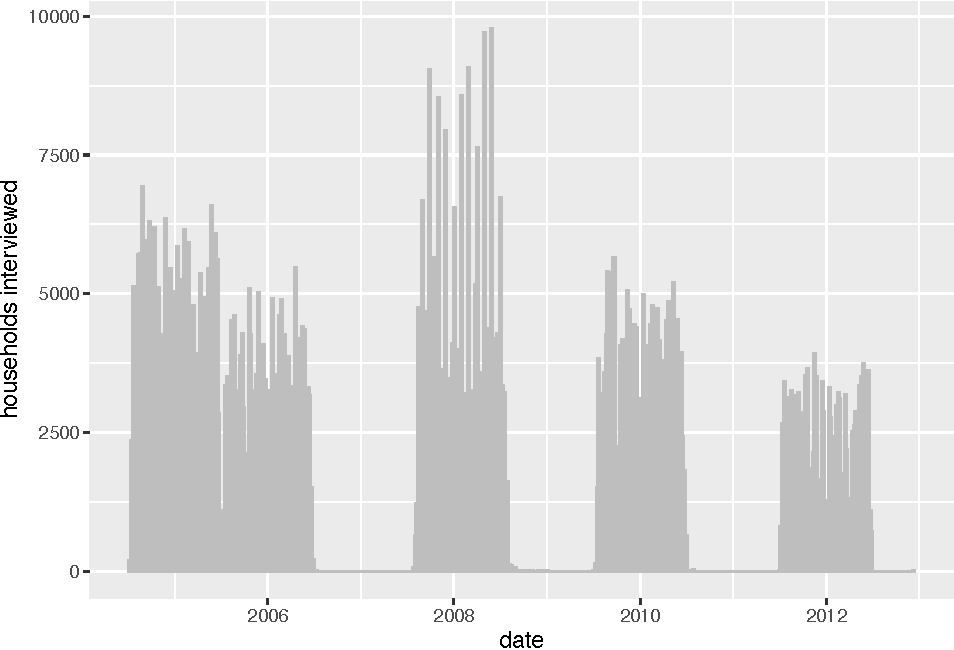
\includegraphics{draft_files/figure-latex/laborplot-1} \caption[Timing of household surveys for the National Sample Survey]{Timing of household surveys for the National Sample Survey}\label{fig:laborplot}\floatfoot*{Note: The histogram shows the distribution of survey dates for the four waves of the National Sample Survey (NSS) for the five waves used in this paper.}
\end{figure}

\FloatBarrier
\newpage

\begin{table}

\caption{\label{tab:labortablemonsoon}Wind direction and labor allocation, monsoon season only}
\centering
\begin{threeparttable}
\begin{tabular}[t]{>{\raggedright\arraybackslash}p{3cm}>{\centering\arraybackslash}p{1.5cm}>{\centering\arraybackslash}p{1.5cm}>{\centering\arraybackslash}p{1.5cm}>{\centering\arraybackslash}p{1.5cm}>{\centering\arraybackslash}p{1.5cm}>{\centering\arraybackslash}p{1.5cm}}
\toprule
  & all & all & self & wage & farm & non-farm\\
\midrule
wind & -0.120*** & -0.119** & -0.067 & -0.052 & 0.025 & -0.144**\\
 & (0.046) & (0.046) & (0.042) & (0.045) & (0.036) & (0.062)\\
controls & No & Yes & Yes & Yes & Yes & Yes\\
\textbf{fixed effects:} & \textbf{} & \textbf{} & \textbf{} & \textbf{} & \textbf{} & \textbf{}\\
district & Yes & Yes & Yes & Yes & Yes & Yes\\
state-month & Yes & Yes & Yes & Yes & Yes & Yes\\
\textbf{DV mean} & \textbf{3.324} & \textbf{3.324} & \textbf{1.883} & \textbf{1.441} & \textbf{0.810} & \textbf{2.513}\\
observations & 359,652 & 359,576 & 359,576 & 359,576 & 359,576 & 359,576\\
\midrule
\bottomrule
\end{tabular}
\begin{tablenotes}[para]
\item Note: Standard errors are in parentheses and are clustered at the district level. Control variables include female, age, age squared, and (years of) education. * p<0.10 ** p<0.05 *** p<0.01
\end{tablenotes}
\end{threeparttable}
\end{table}

\FloatBarrier
\newpage

\begin{table}

\caption{\label{tab:labortablewinter}Wind direction and labor allocation, winter season only}
\centering
\begin{threeparttable}
\begin{tabular}[t]{>{\raggedright\arraybackslash}p{3cm}>{\centering\arraybackslash}p{1.5cm}>{\centering\arraybackslash}p{1.5cm}>{\centering\arraybackslash}p{1.5cm}>{\centering\arraybackslash}p{1.5cm}>{\centering\arraybackslash}p{1.5cm}>{\centering\arraybackslash}p{1.5cm}}
\toprule
  & all & all & self & wage & farm & non-farm\\
\midrule
wind & -0.012 & -0.032 & -0.026 & -0.006 & -0.020 & -0.012\\
 & (0.040) & (0.037) & (0.040) & (0.028) & (0.030) & (0.036)\\
controls & No & Yes & Yes & Yes & Yes & Yes\\
\textbf{fixed effects:} & \textbf{} & \textbf{} & \textbf{} & \textbf{} & \textbf{} & \textbf{}\\
district & Yes & Yes & Yes & Yes & Yes & Yes\\
state-month & Yes & Yes & Yes & Yes & Yes & Yes\\
\textbf{DV mean} & \textbf{3.339} & \textbf{3.339} & \textbf{1.865} & \textbf{1.474} & \textbf{0.790} & \textbf{2.550}\\
observations & 375,956 & 375,883 & 375,883 & 375,883 & 375,883 & 375,883\\
\midrule
\bottomrule
\end{tabular}
\begin{tablenotes}[para]
\item Note: Standard errors are in parentheses and are clustered at the district level. Control variables include female, age, age squared, and (years of) education. The outcome in each regression is days worked in the previous seven days. * p<0.10 ** p<0.05 *** p<0.01
\end{tablenotes}
\end{threeparttable}
\end{table}

\FloatBarrier
\newpage

\begin{table}

\caption{\label{tab:labortableoldstate}Wind direction and labor allocation, heterogeneity by age}
\centering
\begin{threeparttable}
\begin{tabular}[t]{>{\raggedright\arraybackslash}p{4cm}>{\centering\arraybackslash}p{1.5cm}>{\centering\arraybackslash}p{1.5cm}>{\centering\arraybackslash}p{1.5cm}>{\centering\arraybackslash}p{1.5cm}>{\centering\arraybackslash}p{1.5cm}}
\toprule
  & all & self & wage & farm & non-farm\\
\midrule
wind & 0.100*** & 0.117*** & -0.018 & 0.026 & 0.074***\\
 & (0.027) & (0.029) & (0.026) & (0.024) & (0.028)\\
wind times age>=38 & -0.203*** & -0.201*** & -0.002 & -0.070*** & -0.133***\\
 & (0.037) & (0.032) & (0.039) & (0.018) & (0.031)\\
controls & Yes & Yes & Yes & Yes & Yes\\
\textbf{fixed effects:} & \textbf{} & \textbf{} & \textbf{} & \textbf{} & \textbf{}\\
district-year-month & Yes & Yes & Yes & Yes & Yes\\
\midrule
observations & 898,856 & 898,856 & 898,856 & 898,856 & 898,856\\
\bottomrule
\end{tabular}
\begin{tablenotes}[para]
\item Note: Standard errors are in parentheses and are clustered at the district level. Control variables include female, age, age squared, and (years of) education. The outcome in each regression is days worked in the previous seven days. * p<0.10 ** p<0.05 *** p<0.01
\end{tablenotes}
\end{threeparttable}
\end{table}

\FloatBarrier
\newpage

\begin{table}

\caption{\label{tab:wagestable}Wind direction and wages}
\centering
\begin{threeparttable}
\begin{tabular}[t]{>{\raggedright\arraybackslash}p{3cm}>{\centering\arraybackslash}p{1.5cm}>{\centering\arraybackslash}p{1.5cm}>{\centering\arraybackslash}p{1.5cm}}
\toprule
  & farm & non-farm & all\\
\midrule
wind & 0.037 & 0.010 & 0.009\\
 & (0.031) & (0.010) & (0.011)\\
controls & Yes & Yes & Yes\\
\textbf{fixed effects:} & \textbf{} & \textbf{} & \textbf{}\\
district & Yes & Yes & Yes\\
year & Yes & Yes & Yes\\
\textbf{varying slopes:} & \textbf{} & \textbf{} & \textbf{}\\
year (by district) & Yes & Yes & Yes\\
\midrule
observations & 16,534 & 149,973 & 133,526\\
\bottomrule
\end{tabular}
\begin{tablenotes}[para]
\item Note: Standard errors are in parentheses and are clustered at the district level. Control variables include female, age, age squared, and (years of) education. The outcome in each regression is the daily wage (log Rs per day). * p<0.10 ** p<0.05 *** p<0.01
\end{tablenotes}
\end{threeparttable}
\end{table}

\end{document}
